% Ejemplo de diagrama de Bode con pgfplots. Reemplazar la expresión analítica por datos exportados de la simulación:
%   \addplot table[col sep=comma, x=f, y=dB] {sources/bode_pasa_bajos.csv};
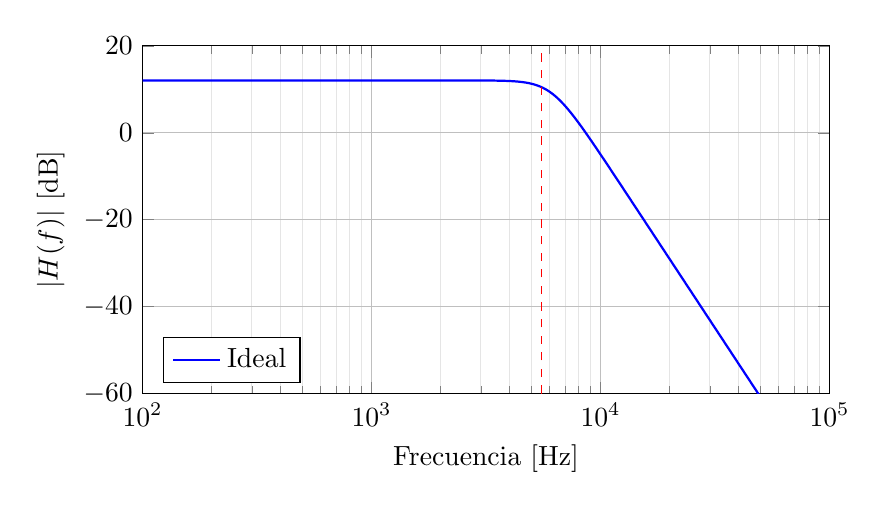
\begin{tikzpicture}
  \begin{semilogxaxis}[
      width=0.85\textwidth, height=6cm,
      xlabel={Frecuencia [Hz]}, ylabel={$|H(f)|$ [dB]},
      xmin=100, xmax=100000, ymin=-60, ymax=20,
      grid=both, minor grid style={gray!20}, major grid style={gray!50},
      legend pos=south west, legend cell align=left,
      samples=200, domain=100:100000,
    ]
    % Butterworth orden 4, f_c = 6,14 kHz, ganancia 4 V/V (12 dB)
    \addplot[blue, thick] {20*log10(4) - 10*log10(1 + (x/6140)^8)};
    \addlegendentry{Ideal}
    \draw[dashed, red] (axis cs:5500,-60) -- (axis cs:5500,20) node[above, black] {\scriptsize $f_p$};
  \end{semilogxaxis}
\end{tikzpicture}
